\begin{center}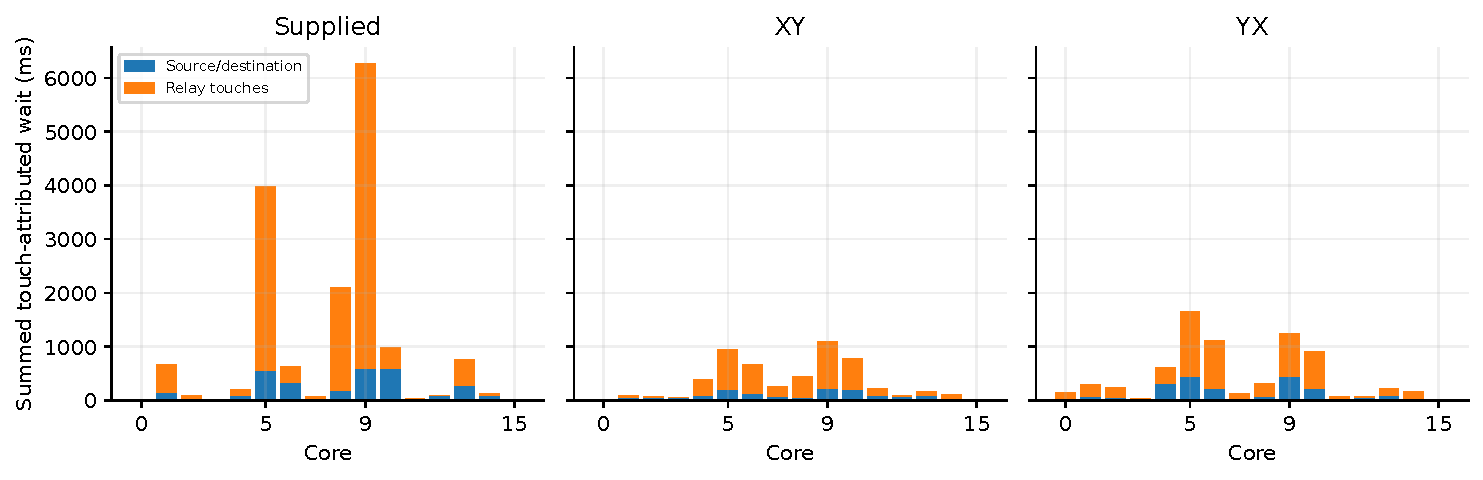
\includegraphics[width=\linewidth,height=0.37\textheight,keepaspectratio]{figures/percore.pdf}\captionof{figure}{Dynamic waiting attributed to endpoint and relay touches, averaged over five physics seeds. A hop touches two cores, so these sums are not wall-clock latency and can count one request twice.}\end{center}

\begin{center}\small
\begin{longtable}{lrrr}
\caption{Complete core-wise values underlying the figure, in ms.}\\
\toprule
Core & Supplied end/relay & XY end/relay & YX end/relay \\
\midrule\endfirsthead
\toprule
Core & Supplied end/relay & XY end/relay & YX end/relay \\
\midrule\endhead
0 & 20.2 / 0.0 & 12.2 / 11.0 & 36.0 / 102.2 \\
1 & 139.4 / 523.6 & 61.3 / 30.2 & 75.0 / 229.5 \\
2 & 36.9 / 63.8 & 49.2 / 24.3 & 51.2 / 197.2 \\
3 & 6.2 / 0.0 & 54.5 / 4.4 & 21.2 / 17.4 \\
4 & 99.3 / 112.9 & 91.5 / 289.2 & 320.5 / 290.7 \\
5 & 561.0 / 3420.2 & 194.3 / 744.6 & 440.4 / 1206.1 \\
6 & 338.0 / 301.4 & 128.8 / 543.7 & 221.9 / 889.5 \\
7 & 40.2 / 36.2 & 69.2 / 198.4 & 41.9 / 82.4 \\
8 & 193.7 / 1912.4 & 53.1 / 397.7 & 78.0 / 240.3 \\
9 & 585.5 / 5675.4 & 222.5 / 867.5 & 436.6 / 800.9 \\
10 & 587.7 / 396.8 & 202.1 / 568.6 & 215.4 / 690.6 \\
11 & 32.7 / 11.0 & 85.3 / 141.4 & 44.7 / 32.0 \\
12 & 90.0 / 0.0 & 69.7 / 26.1 & 60.0 / 10.4 \\
13 & 283.5 / 484.0 & 98.9 / 74.8 & 99.1 / 125.6 \\
14 & 82.7 / 47.9 & 31.8 / 76.7 & 30.0 / 141.2 \\
15 & 4.8 / 4.6 & 9.1 / 17.3 & 5.9 / 9.0 \\
\bottomrule\end{longtable}\end{center}
{\footnotesize \href{https://github.com/sanjeevkrishnaa/Compiler-Driven-ACE/blob/codex/ace-scheduler-correctness/docs/latex/oct25_pre_golden/data/per_core_wait.csv}{Complete CSV: per\_core\_wait}. }
